%% Estructura principal para un reporte de Trabajos intersemanales CIRCAE %%
\documentclass[a4paper]{IEEEtran} %tamaño del papel y el tipo de transcripción que será IEEE
\usepackage[utf8]{inputenc} %el tipo de codificación que incluye símbolos como la tilde
\usepackage[spanish]{babel} % hacemos que nuestro documentación vaya en español
\usepackage{cite} % citas bibliográficas
\usepackage{graphicx} %gráficos, usaremos solo .jpg o .png con estándares que ya veremos
\usepackage{subfigure}
\usepackage{url}
\usepackage{amsmath}
\usepackage{booktabs} 
\providecommand{\keywords}[1]{\textbf{\textit{Términos Clave---}} #1}
\begin{document}

\title{WILKINSON POWER DIVIDER SIMULATION}
\author{Hanan Ronaldo Quispe Condori, CIRCAE Student Member}
\markboth{INFORME CIRCAE 2019-08-05-G1-P3-001}{} % Codigo del informe que corresponde a: semestre | mes | dia | numero de grupo con la G antepuesta | numero de proyecto con la P antepuesta | número de informe
\maketitle
\begin{abstract}
El divisor de potencia de Wilkinson es un dispositivo pasivo con todos sus puertos emparejados,no tiene perdidas cuando el puerto de entrada se excita y los puertos de salida estan aislados,esta simulacion imlementara un divisor de potencia para el rango de frecuencia de 0 a 2GHz.
\end{abstract}
\begin{figure}[h]
    \centering
        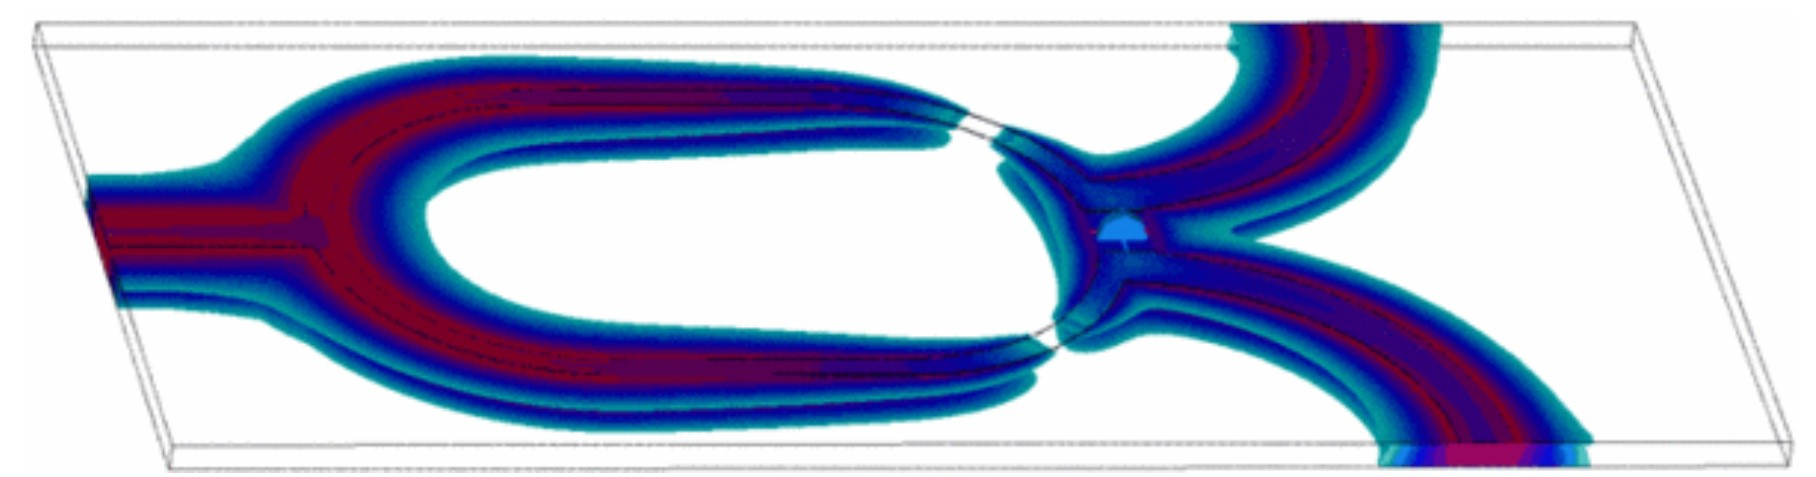
\includegraphics[width=8cm]{imagenes/img2}
        \caption{E-field phase animation of a Wilkinson power divider.}
        \label{fig E-field phase animation of a Wilkinson power divider.}
\end{figure}
\section{Problema}
La division de una señal de entrada en señales de salida equiamplitud y equifase se logra con un divisor tipo T o un divisor resistivo,pero estos presentan la limitacion de tan solo poseer un numero par de salidas, por ejemplo en caso se necesitaran usar 9 salidas, un divisor de 16 salidas tendria que ser utlizado, esto produciria disipación de potencia innecesaria,el divisor de potencia de Wilkinson soluciona este problema.
\section{Fundamento Teórico}
Los divisores de potencia poseen matrices de dispersión que nos diran cual sera el comportamiento de dicho divisor, los calculos matemáticos sobre esta matriz nos diran que es lo que se puede o se puede hacer con un determinado divisor, la matriz den dispersión de del modelo a simular se muestra en la figura 2.\\
\begin{figure}[h]
    \centering
        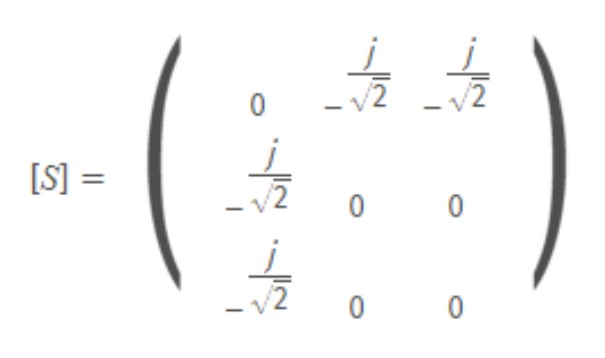
\includegraphics[width=6cm]{imagenes/img1}
        \caption{Scattering matrix.}
        \label{fig.}
\end{figure}
Para analizar totalmente esta estructura realizaremos un analisis "par-impar",dicho analisis se realizara como se muestran en la figuras número tres y número cuatro 
\begin{figure}[h]
    \centering
        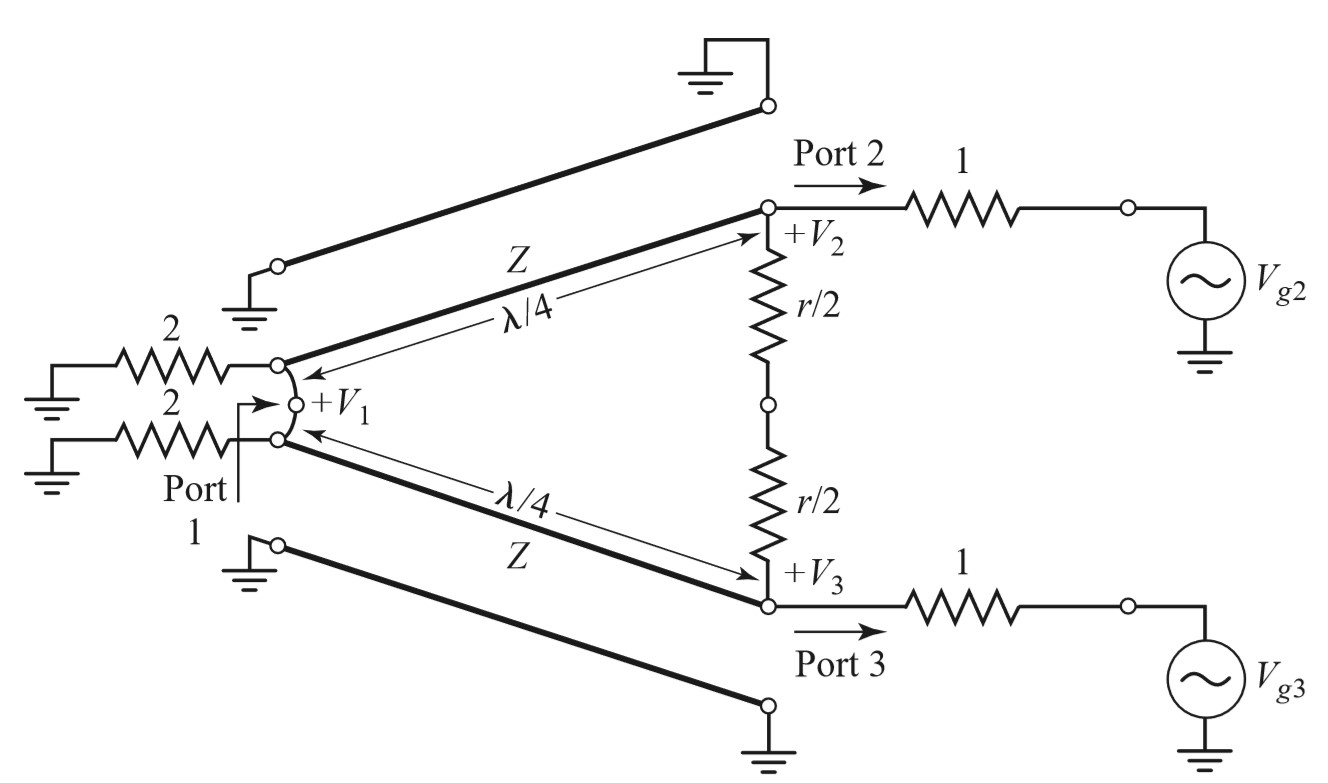
\includegraphics[width=8cm]{imagenes/img3}
        \caption{Diagrama Esquematico del divisor de potencia de Wilkinson.}
        \label{fig.}
\end{figure}
\begin{figure}[h]
    \centering
        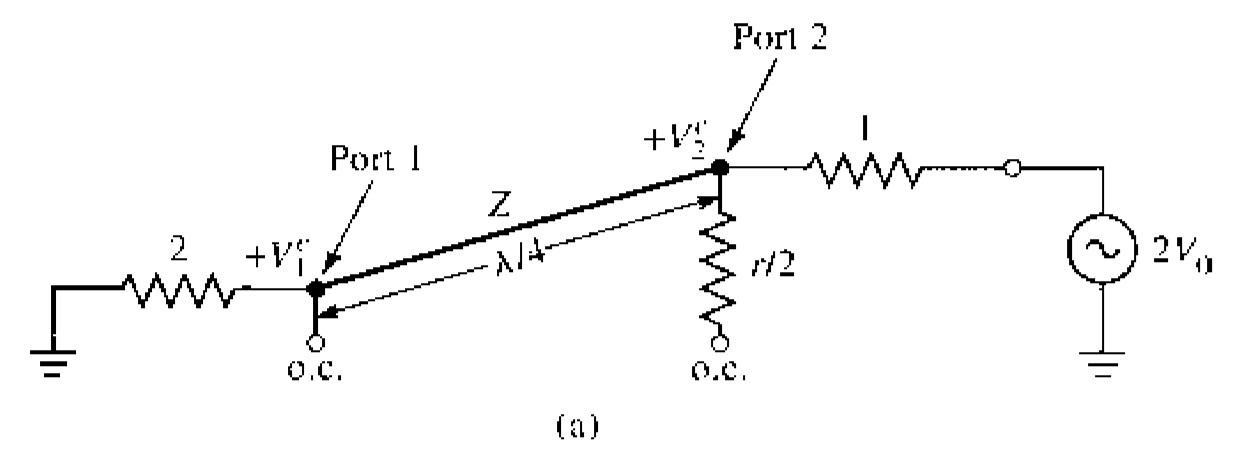
\includegraphics[width=8cm]{imagenes/img4}
        \caption{Analisis Par-Impar.}
        \label{fig.}
\end{figure}
\newline
\newline
\newline
\newline
\newline
\section{El modelo}
Se utilizará CST Studio Suite para el modelamiento de este divisor,los datos a utilizar en la simulación estan dados en el cuadro.
\begin{table}[h]
\begin{tabular}{@{}lll@{}}
\toprule
Parametro & Valor    & Descripción                               \\ \midrule
h         & 1.2 mm   & Grosor del Substrato                      \\
eps\_r    & 4.3      & Permitividad del Substrato                \\
t         & 0.035 mm & Espesor de metalización                   \\ \midrule
W50       & 2.35 mm  & 50 Ohms (Z0) Anchura de linea               \\
W70       & 1.23 mm  & 70.71 Omhs (Z0$\sqrt{2}$)                          \\
l70       & 42.54 mm & Longitud de Lambda / 4 del ancho de línea Z0$\sqrt{2}$\\ \bottomrule
\end{tabular}
\end{table}

%La bibliografía:
\bibliographystyle{ieeetr}
\bibliography{bibliografia}

\end{document}
